\documentclass[12pt]{article}

% Layout
\usepackage[a4paper, margin=1in]{geometry}
\usepackage{setspace}

% Graphics & figures
\usepackage{graphicx}
\usepackage{xcolor}
\usepackage{pgfgantt}
\usepackage{tikz}
% Links (always last)
\usepackage{hyperref}

\hypersetup{
    colorlinks=true,
    urlcolor=blue,
    linkcolor=black,
    citecolor=black
}

\begin{document}

\onehalfspacing

% -------------------- TITLE PAGE --------------------

\begin{titlepage}

\begin{center}

{\large \textbf{Hawassa University}}\\[0.3cm]
{\normalsize Institute of Technology}\\[0.3cm]
{\normalsize Faculty of Informatics}\\[0.3cm]
{\normalsize Department of Computer Science}

\vspace{2cm}

{\LARGE \textbf{Research Proposal}}\\[0.8cm]

{\Large \textbf{Development of a Web-Based Bug Tracking and Reporting System}}

\vspace{2.5cm}

\end{center}

\noindent
\begin{tabular}{ll}
\textbf{Student Name:} & Ebsitu Berhanu \\
\textbf{ID Number:} & 1855/16 \\
\textbf{Course:} & Research Methods in Computer Science (CoSc3101) \\
\textbf{Instructor:} & Birhane.B \\
\textbf{Submission Date:} & May 1, 2026 \\
\end{tabular}

\vfill

\begin{center}
{\normalsize Hawassa, Ethiopia}
\end{center}

\end{titlepage}

\newpage
\tableofcontents
\newpage

% =====================================================
% 1. INTRODUCTION
% =====================================================

\section{Introduction}

Software systems have become an essential part of modern society, powering applications in healthcare, finance, education, and communication. As these systems grow in complexity, they are increasingly prone to software bugs that affect performance, reliability, and user experience. Efficient detection, reporting, and tracking of these bugs is therefore a critical requirement in software engineering.

The rise of interconnected systems such as the Internet of Things (IoT) further increases the importance of reliable software. IoT devices enable unprecedented connectivity by integrating smart devices into everyday environments. In 2020, approximately 5.8 billion IoT endpoints were in use worldwide. However, the widespread deployment of these devices introduces significant security risks, as they are highly vulnerable to software bugs and cyberattacks. Reports indicate that around 57\% of IoT devices are exposed to medium or high-severity vulnerabilities, making them attractive targets for attackers. This highlights the growing need for robust bug tracking and management systems to ensure system reliability and security.

Despite the availability of existing bug tracking tools, many organizations still rely on inefficient methods such as spreadsheets, emails, or complex systems that are difficult to use for small development teams. This creates challenges in communication, bug prioritization, and timely resolution.

Therefore, this project proposes the development of a simple, efficient, and web-based bug tracking and reporting system that improves collaboration between developers and testers while ensuring effective bug management.

% =====================================================
% 2. PROBLEM STATEMENT
% =====================================================

\section{Problem Statement}

In modern software development environments, effective bug tracking and reporting is a critical component for ensuring software quality, maintainability, and timely delivery. However, many development teams—especially small and medium-scale teams—still rely on fragmented or inefficient bug management approaches such as email communication, spreadsheets, or loosely connected tools.

These approaches introduce several challenges, including inconsistent bug documentation, delayed issue resolution, lack of centralized tracking, and poor coordination between developers, testers, and project managers. As a result, software defects may remain unresolved for longer periods, negatively affecting system reliability and user satisfaction.
 Although existing bug tracking systems such as Bugzilla and similar platforms provide comprehensive functionalities, they are often complex to configure, resource-intensive, and not optimized for lightweight or beginner-friendly usage. On the other hand, advanced AI-based and automated bug detection solutions improve accuracy but require significant computational resources and large datasets, making them impractical for basic or academic-level systems.

Therefore, there is a need for a simple, efficient, and user-friendly web-based bug tracking and reporting system that provides essential bug management functionalities such as reporting, tracking, assignment, and status monitoring while maintaining ease of use and system efficiency.

% =====================================================
% 3. OBJECTIVES
% =====================================================

\section{Objectives}

\subsection{General Objective}
To design and develop a simple, efficient, and user-friendly web-based bug tracking and reporting system that improves software bug management in small and medium-scale development environments.

\subsection{Specific Objectives}

\begin{itemize}
    \item To analyze existing bug tracking systems and identify their limitations in usability, complexity, and scalability, in order to inform the design of an improved solution.

    \item To design and implement a web-based bug tracking system that supports efficient bug reporting, tracking, assignment, and real-time status monitoring through role-based functionality.

    \item To evaluate the developed system in terms of usability, performance, and bug tracking efficiency compared to existing lightweight bug tracking solutions.
\end{itemize}
% =====================================================
% 4. LITERATURE REVIEW
% =====================================================

\section{Literature Review}

Recent research in software engineering has focused on improving bug tracking systems, automation, and software quality assurance through both traditional and intelligent approaches.

Gopal et al. (2022) proposed \textit{Bugtrac} \cite{singh2023bugzilla}, an improved bug tracking system designed to enhance usability and streamline defect management. While the system improves user interaction compared to traditional tools like Bugzilla, it still lacks wide adoption in real-world development environments, limiting its practical impact.

Singh et al. (2023) analyzed the Bugzilla bug tracking system \cite{gopal2022bugtrac} and found that it provides strong support for bug lifecycle management and collaboration among developers. However, the study highlighted that Bugzilla is often complex and less suitable for small-scale or beginner development teams due to its heavy configuration requirements.

Vadia et al. (2024)  introduced an automated bug testing framework \cite{vadia2024playwright} using Playwright integrated with backend APIs. Their work improves testing efficiency in modern web applications, especially in cloud-based environments. However, the focus is mainly on automated testing rather than full lifecycle bug tracking and management.

Ndlovu et al. (2024) conducted a systematic review of artificial intelligence-based software fault detection techniques  \cite{ndlovu2024ai}. Their findings show that AI significantly improves accuracy, scalability, and automation in identifying software faults. However, most AI-based approaches are computationally expensive and require large datasets, making them unsuitable for lightweight systems.

Patel (2025) proposed a neural network-based bug detection model\cite{patel2025ml} using machine learning techniques, achieving high accuracy in defect prediction. Despite its strong performance, the model depends heavily on large-scale datasets and is more suitable for prediction rather than real-time bug tracking systems.

Overall, existing studies demonstrate significant progress in bug tracking, automation, and defect prediction. However, most solutions are either too complex, resource-intensive, or focused only on specific stages of the software development lifecycle. This creates a research gap for a simple, lightweight, and user-friendly web-based bug tracking system that supports full bug lifecycle management efficiently.
\subsection{Research Gap Synthesis}

The reviewed literature demonstrates significant advancements in bug tracking systems, automated testing frameworks, and artificial intelligence-based fault detection techniques. Studies such as Bugzilla and Bugtrac focus on structured bug lifecycle management, while modern tools like Playwright introduce automation in software testing. Additionally, AI-based approaches have improved defect prediction accuracy using machine learning and neural networks.

However, despite these advancements, several limitations remain. Traditional systems like Bugzilla are often complex and require extensive configuration, making them unsuitable for small-scale or beginner development teams. Automated testing tools primarily focus on test execution rather than complete bug lifecycle management. Similarly, AI-based solutions achieve high accuracy but depend heavily on large datasets and computational resources, limiting their applicability in lightweight environments.

Furthermore, most existing systems are either too specialized or fragmented, addressing only specific stages of software quality assurance rather than providing a complete and integrated bug tracking solution. This creates a gap between advanced, resource-intensive systems and simple, user-friendly tools required by small development teams.

Therefore, this research aims to fill this gap by developing a lightweight, web-based bug tracking and reporting system that integrates essential functionalities such as bug reporting, assignment, tracking, and status monitoring. The proposed system emphasizes simplicity, usability, and efficiency, making it suitable for educational environments and small to medium-scale software development teams. By combining essential features into a unified platform, the system addresses the limitations of existing solutions while maintaining ease of use and low computational requirements.
% =====================================================
% 5. SYNTHESIS MATRIX
% =====================================================

\section{Synthesis Matrix}

\begin{table}[h!]
\centering
\renewcommand{\arraystretch}{1.5}

\begin{tabular}{|p{2.5cm}|p{3cm}|p{3cm}|p{3cm}|p{3cm}|}
\hline
\textbf{Author} & \textbf{Method} & \textbf{Dataset} & \textbf{Performance Metric} & \textbf{Limitation} \\
\hline

Singh et al. & Bugzilla analysis & Real-world bug tracking records & Bug lifecycle efficiency & Complex configuration for small teams \\
\hline

Gopal et al. & System design (Bugtrac) & Simulated bug reports dataset & Usability improvement & Low adoption in industry \\
\hline

Vadia et al. & Automation testing (Playwright) & Web application test cases & Testing speed and automation efficiency & Not full bug tracking system \\
\hline

Ndlovu et al. & AI-based fault detection review & Multiple research datasets & Accuracy of fault detection models & High computational cost, theoretical focus \\
\hline

Patel (2025) & Neural network prediction model & Large-scale software defect datasets & 91\% prediction accuracy & Requires large training datasets \\
\hline

\end{tabular}
\end{table}
\section{Methodology}

This research adopts a structured Software Development Life Cycle (SDLC) approach to design, implement, and evaluate a web-based bug tracking and reporting system. The methodology ensures systematic development, testing, and validation of the proposed system.
\subsection{Data Strategy and Preprocessing}

Since this project focuses on a web-based bug tracking system rather than a machine learning model, the dataset is based on structured bug report records generated within the system. These records include fields such as bug title, description, priority level, status, assigned developer, and timestamps.

The dataset will be created and stored in a MySQL relational database and will be used to simulate real-world software development environments.

\textbf{Data Preprocessing Steps:}
\begin{itemize}
    \item Data Validation: Ensuring all bug reports contain required fields before submission.
    \item Data Cleaning: Removing duplicate or incomplete bug entries.
    \item Data Formatting: Standardizing priority levels (Low, Medium, High, Critical).
    \item Data Normalization: Organizing data into relational tables to reduce redundancy.
    \item Status Encoding: Converting bug states (Open, In Progress, Resolved) into structured values.
\end{itemize}

This structured dataset allows efficient storage, retrieval, and analysis of bug reports within the system.
% -----------------------------------------------------
\subsection{System Design Approach}

The proposed system is designed using a client-server architecture to ensure modularity, scalability, and maintainability. The system is divided into three main layers:

\begin{itemize}
    \item \textbf{Presentation Layer (Frontend):} Handles user interaction using HTML, CSS, and JavaScript. It allows users to submit bug reports, view status updates, and interact with the system.

    \item \textbf{Application Layer (Backend):} Handles core business logic such as authentication, bug processing, role management, and workflow control. It is implemented using PHP or Node.js.

    \item \textbf{Data Layer (Database):} Responsible for persistent storage of system data including users, bug reports, comments, and history logs using MySQL.
\end{itemize}

\vspace{0.5cm}

\begin{center}
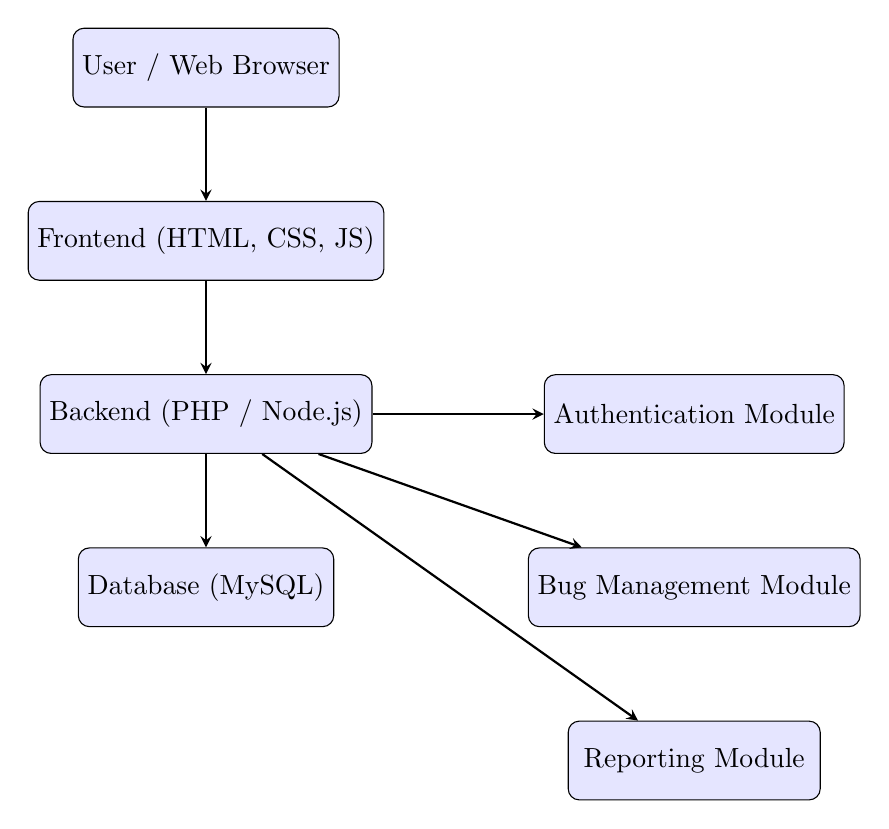
\begin{tikzpicture}[
    node distance=2.2cm,
    box/.style={rectangle, rounded corners, minimum width=3.2cm, minimum height=1cm, text centered, draw=black, fill=blue!10},
    arrow/.style={thick,->,>=stealth}
]

% Nodes
\node (user) [box] {User / Web Browser};

\node (frontend) [box, below of=user] {Frontend (HTML, CSS, JS)};

\node (backend) [box, below of=frontend] {Backend (PHP / Node.js)};

\node (db) [box, below of=backend] {Database (MySQL)};

% Flow arrows
\draw [arrow] (user) -- (frontend);
\draw [arrow] (frontend) -- (backend);
\draw [arrow] (backend) -- (db);

% Backend internal modules
\node (auth) [box, right of=backend, xshift=4cm] {Authentication Module};
\node (bug) [box, below of=auth] {Bug Management Module};
\node (report) [box, below of=bug] {Reporting Module};

\draw [arrow] (backend) -- (auth);
\draw [arrow] (backend) -- (bug);
\draw [arrow] (backend) -- (report);

\end{tikzpicture}
\end{center}
\subsection{System Architecture}

The system follows a three-tier architecture model consisting of the user interface, application server, and database server. Users interact with the frontend interface, which communicates with the backend server through HTTP requests. The backend processes requests, applies business logic, and interacts with the database to store or retrieve data.

This architecture ensures separation of concerns, scalability, and maintainability of the system.

% -----------------------------------------------------
\subsection{Data Collection and Management}

The system handles structured data related to bug tracking operations. The main data entities include user information, bug reports, assignment records, and status updates.

Data will be stored in normalized relational tables to reduce redundancy and ensure data consistency. Input validation and authentication mechanisms will be implemented to ensure data integrity and security.

% -----------------------------------------------------
\subsection{Development Tools and Technologies}

The following technologies are selected for system development:

\begin{itemize}
    \item \textbf{Frontend:} HTML, CSS, JavaScript (for responsive user interface design)
    \item \textbf{Backend:} PHP or Node.js (for server-side logic and request handling)
    \item \textbf{Database:} MySQL (for structured data storage and management)
\end{itemize}
These tools are selected due to their simplicity, reliability, and suitability for developing lightweight and scalable web-based applications.
\subsection{Tool Justification}

The selection of technologies in this project is based on simplicity, performance, and suitability for lightweight web applications.

\textbf{HTML, CSS, JavaScript:} These technologies are used for frontend development because they are standard web technologies that provide responsive and interactive user interfaces without requiring additional dependencies.

\textbf{PHP / Node.js:} The backend is implemented using either PHP or Node.js due to their efficiency in handling server-side logic, authentication, and database communication. PHP is widely supported in academic environments, while Node.js provides modern asynchronous processing capabilities.

\textbf{MySQL:} MySQL is chosen as the database management system because it is reliable, widely used, and suitable for structured relational data such as bug reports, user accounts, and system logs.

These tools are selected over more complex frameworks because the goal of this project is to develop a lightweight, easy-to-deploy, and efficient bug tracking system suitable for small and medium-scale development teams.

% -----------------------------------------------------
\subsection{Evaluation Methodology}

The performance of the proposed system will be evaluated using both qualitative and quantitative metrics to ensure its effectiveness and usability compared to existing bug tracking systems.

\begin{itemize}
    \item \textbf{Bug Resolution Time:} Measures the average time required to identify, assign, and resolve reported bugs within the system.

    \item \textbf{System Response Time:} Evaluates the efficiency of the system in processing user requests and database transactions.

    \item \textbf{Usability:} Assessed based on user feedback regarding interface simplicity, accessibility, and ease of navigation.

    \item \textbf{Tracking Efficiency:} Measures the accuracy and effectiveness of bug reporting, updating, and monitoring processes within the system.
\end{itemize}

These metrics will be used to evaluate the overall performance of the proposed system and compare it with existing lightweight bug tracking solutions in terms of efficiency, usability, and responsiveness.
% =====================================================
% 6. PROJECT MANAGEMENT & ETHICS
% =====================================================

\section{Project Management \& Ethics}


% ==========================================

\subsection{Implementation Timeline (Gantt Chart)}

This research follows a structured 5-week implementation schedule, starting from March 24, 2026. The project is divided into major phases including requirement analysis, literature review and system design, system development, testing and integration, and final documentation.

During the initial weeks, emphasis is placed on requirement analysis and literature review to establish a strong foundation for the system design. This is followed by the development phase, where the core functionalities of the system are implemented.

As of this submission (May 1, 2026), the project is approaching its final stages. The remaining time is allocated to testing, system integration, and final documentation. This ensures that all system requirements are satisfied and the project is ready for final evaluation.

\begin{figure}[h!]
\centering
\begin{ganttchart}[
    x unit=1.3cm,
    y unit title=0.7cm,
    y unit chart=0.8cm,
    vgrid,
    hgrid,
    title height=1,
    bar height=0.5,
    bar/.style={fill=blue!60},
    bar label font=\small\bfseries
]{1}{5}

\gantttitle{Project Timeline (Weeks)}{5} \\
\gantttitlelist{1,2,3,4,5}{1} \\

% ONLY PHASES (no subtasks)
\ganttbar{Phase 1: Requirement Analysis \& Planning}{1}{1} \\

\ganttbar{Phase 2: Literature Review \& System Design}{1}{2} \\

\ganttbar{Phase 3: System Development}{2}{4} \\

\ganttbar{Phase 4: Testing \& Integration}{3}{5} \\

\ganttbar{Phase 5: Finalization \& Documentation}{4}{5} \\

\end{ganttchart}
\caption{Weekly Implementation Timeline of the Proposed System}
\end{figure}
\subsection{Ethical Considerations}

The development of the proposed system considers important ethical principles to ensure responsible software engineering practices:

\begin{itemize}
    \item \textbf{Data Privacy:} User information will be securely stored and protected from unauthorized access or misuse.
    
    \item \textbf{Authentication and Security:} Secure login mechanisms will be implemented to prevent unauthorized system access.
    
    \item \textbf{Responsible Data Handling:} All bug reports and system data will be managed ethically, ensuring confidentiality and integrity.
    
    \item \textbf{System Transparency:} The system will ensure that bug tracking processes are transparent and traceable for accountability.
\end{itemize}
% =====================================================
% 7. VERSION CONTROL
% =====================================================
\subsection{Version Control}

Version control is used in this project as a required practice to manage the development process effectively. Git is utilized to track changes in the project files, while GitHub is used as a remote repository for storing and organizing the work.

All source code and documentation are updated regularly using commits to ensure proper tracking of progress. This helps prevent data loss and allows earlier versions of the project to be restored when necessary.

In addition, version control supports better organization of the project by maintaining a clear history of changes and ensuring that the development process remains structured and consistent.

GitHub Repository:
\url{https://github.com/ibsukoo/Web_Based_Bug_Tracking_System_Ebsitu_Berhanu}
\subsection{Standard Workflow}

The project follows a simple version control workflow using Git. Changes are first made in the local development environment and then committed with clear messages to track progress. Afterward, the updates are pushed to the GitHub repository for backup and organization.

This workflow ensures that all modifications are properly recorded, reduces the risk of data loss, and maintains a structured development process throughout the project.
\newpage
% =====================================================
\bibliographystyle{IEEEtran}
\bibliography{references}
\end{document}
